
\chapter{Interface Web}
\label{Logiciel}

Pour délivrer à l'utilisateur une interface agréable et lisible, nous avons décidé de réaliser dans un premier temps une interface web.

\section{Analyse}
\label{sec:uml}

Pour réaliser au mieux cette interface nous avons au préalablement réaliser une phase d'analyse.

Dans la phase d’analyse, on cherche d’abord à bien comprendre et à décrire de façon précise les besoins des utilisateurs ou des clients concernant cette interface. Que souhaitent-ils faire avec le logiciel ? Quelles fonctionnalités veulent-ils ? Pour quel usage ? Comment l’action devrait-elle fonctionner ? C’est ce qu’on appelle \og l’analyse des besoins\fg{}. Après validation de notre compréhension du besoin, nous imaginons la solution. C’est la partie analyse de la solution.

Dans la phase de conception, on apporte plus de détails à la solution et on cherche à clarifier des aspects techniques, tels que l’installation des différentes parties logicielles à installer sur du matériel. Pour réaliser ces deux phases dans un projet informatique, nous utilisons des méthodes, des conventions et des notations. UML fait partie des notations les plus utilisées aujourd’hui. Pour faciliter à nos clients d’obtenir la direction des drones on a créé une interface web qui répond à leur besoin.

\subsection{Uml}

Pour décrire au mieux ce besoin, nous avons commencé par réaliser un cas d'utilisation de l'interface (figure \ref{fig:use_case}).
\begin{figure}[!h]
  \centering
  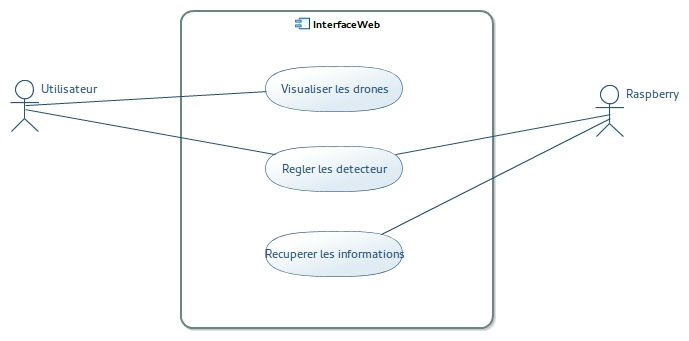
\includegraphics[width=\textwidth]{use_case}
  \caption{Cas d'utilisation de l'interface}
  \label{fig:use_case}
\end{figure}

\newpage
Ensuite, nous avons cherché a réaliser un diagramme de classe de notre interface. Pour cela nous avons défini 3 classes principales:

\begin{itemize}
\item index.php, qui réalise l'affichage dans un navigateur
\item serveur.py, qui récupère les données de chacun des radiogoniomètres
\item client.py, installé sur chaque radiogoniomètres il envoie les données des capteurs à travers un socket au serveur.
\end{itemize}

Le diagrammes de classe de la figure \ref{fig:class}, montre ce fonctionnement.

\begin{figure}[!h]
  \centering
  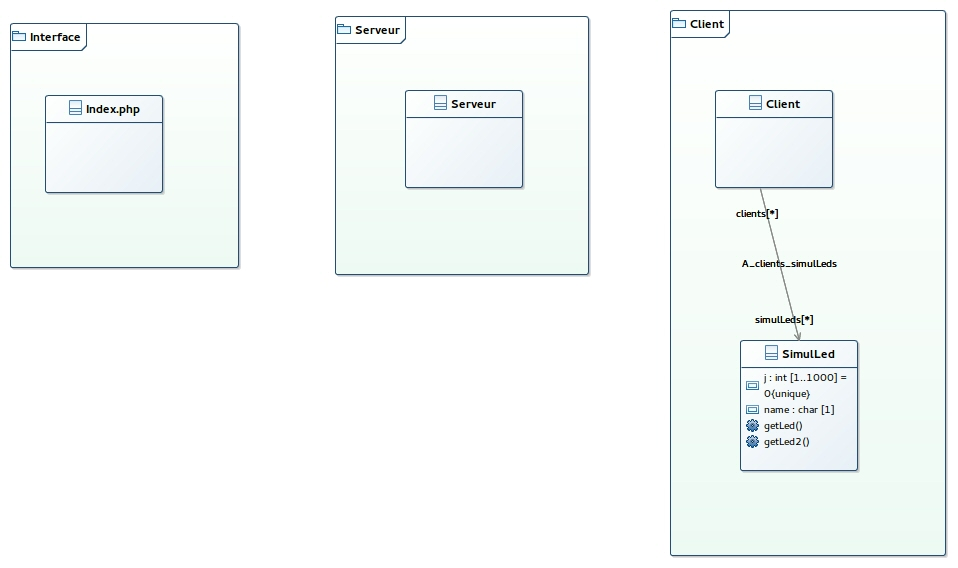
\includegraphics[width=\textwidth]{class_diagram}
  \caption{Diagramme de classe}
  \label{fig:class}
\end{figure}



\section{Conception}

\subsection{Client-Serveur}


\subsection{Web}



\begin{figure}[!h]
  \centering
  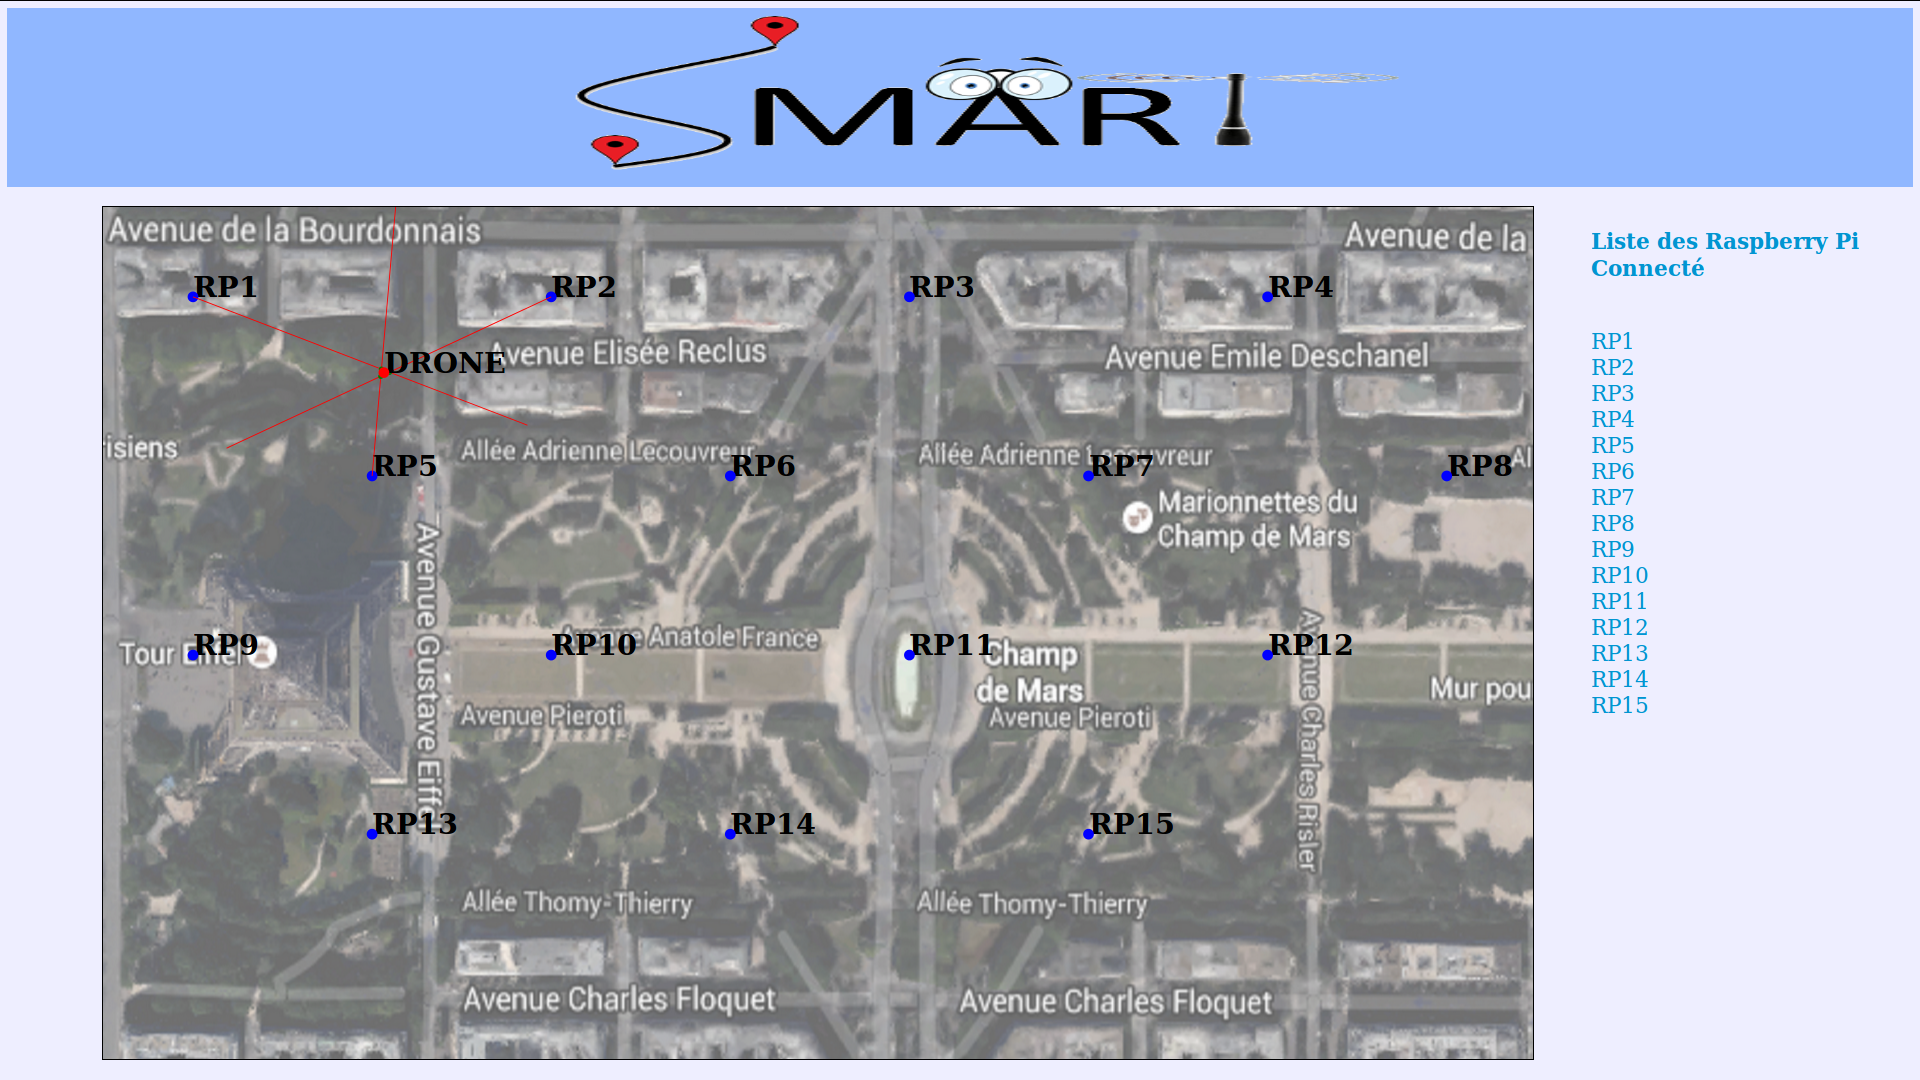
\includegraphics[width=\textwidth]{interface}
  \caption{Interface Web}
  \label{fig:interface}
\end{figure}


%%% Local Variables: 
%%% mode: latex
%%% TeX-master: "../rapport"
%%% End: 
